\documentclass{paper}

%Document Info
\newcommand{\thetitle}{Smart Advisory Generator}
\newcommand{\researchquestion}{}
\newcommand{\theauthor}{Grant Lemons}

\begin{document}
\insertTitlePage
\pagenumbering{roman}
\tableofcontents
\thispagestyle{frontorback}
\newpage
\setcounter{page}{1}
\pagenumbering{arabic}
\justifying

\section{Planning}
\label{sec:planning}
\subsection{Background}
My school organizes the Upper School into small groups of teacher \emph{Advisors} and student \emph{Advisees}.
Advisories are assigned at the beginning of each academic school year and are used for occasions such competitions and trivia.
Teacher advisors also serve the role of guiding advisees on academic matters and representing faculty in parent-teacher conferences.

Each advisory typically has two advisors, one teaching MYP and the other DP.
In order to ensure that advisors will be able to assess a student's academic situation, the school organizes advisories such that at least one of the advisors teaches each student in the advisory.
Other criteria are also kept in mind: each advisory should have an even balance of students from each grade and sex.

Satisfying these requirements creates a challenge for administration at the beginning of each academic school year.
My client, the Dean of Students, is tasked each year with creating these advisories.
Student body growth has made this task increasingly difficult.
After consulting with my client on this issue (\cref{appendix:a}), I realized that this was exactly the type of problem that a computer program would be able to optimize.

\subsection{Solution}
I realized after assessing this issue that the relationships between the data (who teaches whom) were much more important to the problem than the data itself (students and teachers.)
A \textit{graph database}, which emphasizes the relationships between database nodes more than it does the attributes each node possesses, is ideal for this situation.
Each node can still possess attributes, such as name, grade, or sex, but how that data relates to other nodes takes the forefront.
In order to run the business logic required to build the advisories, I decided to create a RESTful backend.
Users interact with the backend via a website built using the Svelte framework.
I chose to architect the product in this manner because I wanted to make the process of using my product as painless as possible, and, had I chosen to create a desktop executable, it would have been less accessible.
Although this problem in particular was faced by my school, I felt that many organizations (schools, companies, or otherwise) might benefit from a generalized version of my product.
As such, I optimized my backend to work in containerized cloud computing environments and to be as fast as possible so it could scale effectively.
To do this, I used the programming language Rust, because I was learning it at the time as I worked on a fairly similar (technology-stack-wise) personal project.
It has several appropriate benefits such as low level performance with modern language features and memory safety through the borrow checker.

\subsection{Success Criteria}
\begin{itemize}
  \itemsep-4pt
  \item The product creates groups of student advisees given certain parameters.
  \item The product allows data to be imported from a spreadsheet.
  \item The product allows for different aspects of generation to be weighted differently.
  \item The client is able to forbid individuals from being placed in an advisory together.
  \item The product stores the client's data between sessions.
\end{itemize}

\section{Design}
\label{sec:design}
\begin{figure}
  
\includegraphics[width=\linewidth]{Login-Mockup}
  \caption{Mockup of login page showed to client}
  \label{design:login}
\end{figure}
\begin{figure}
  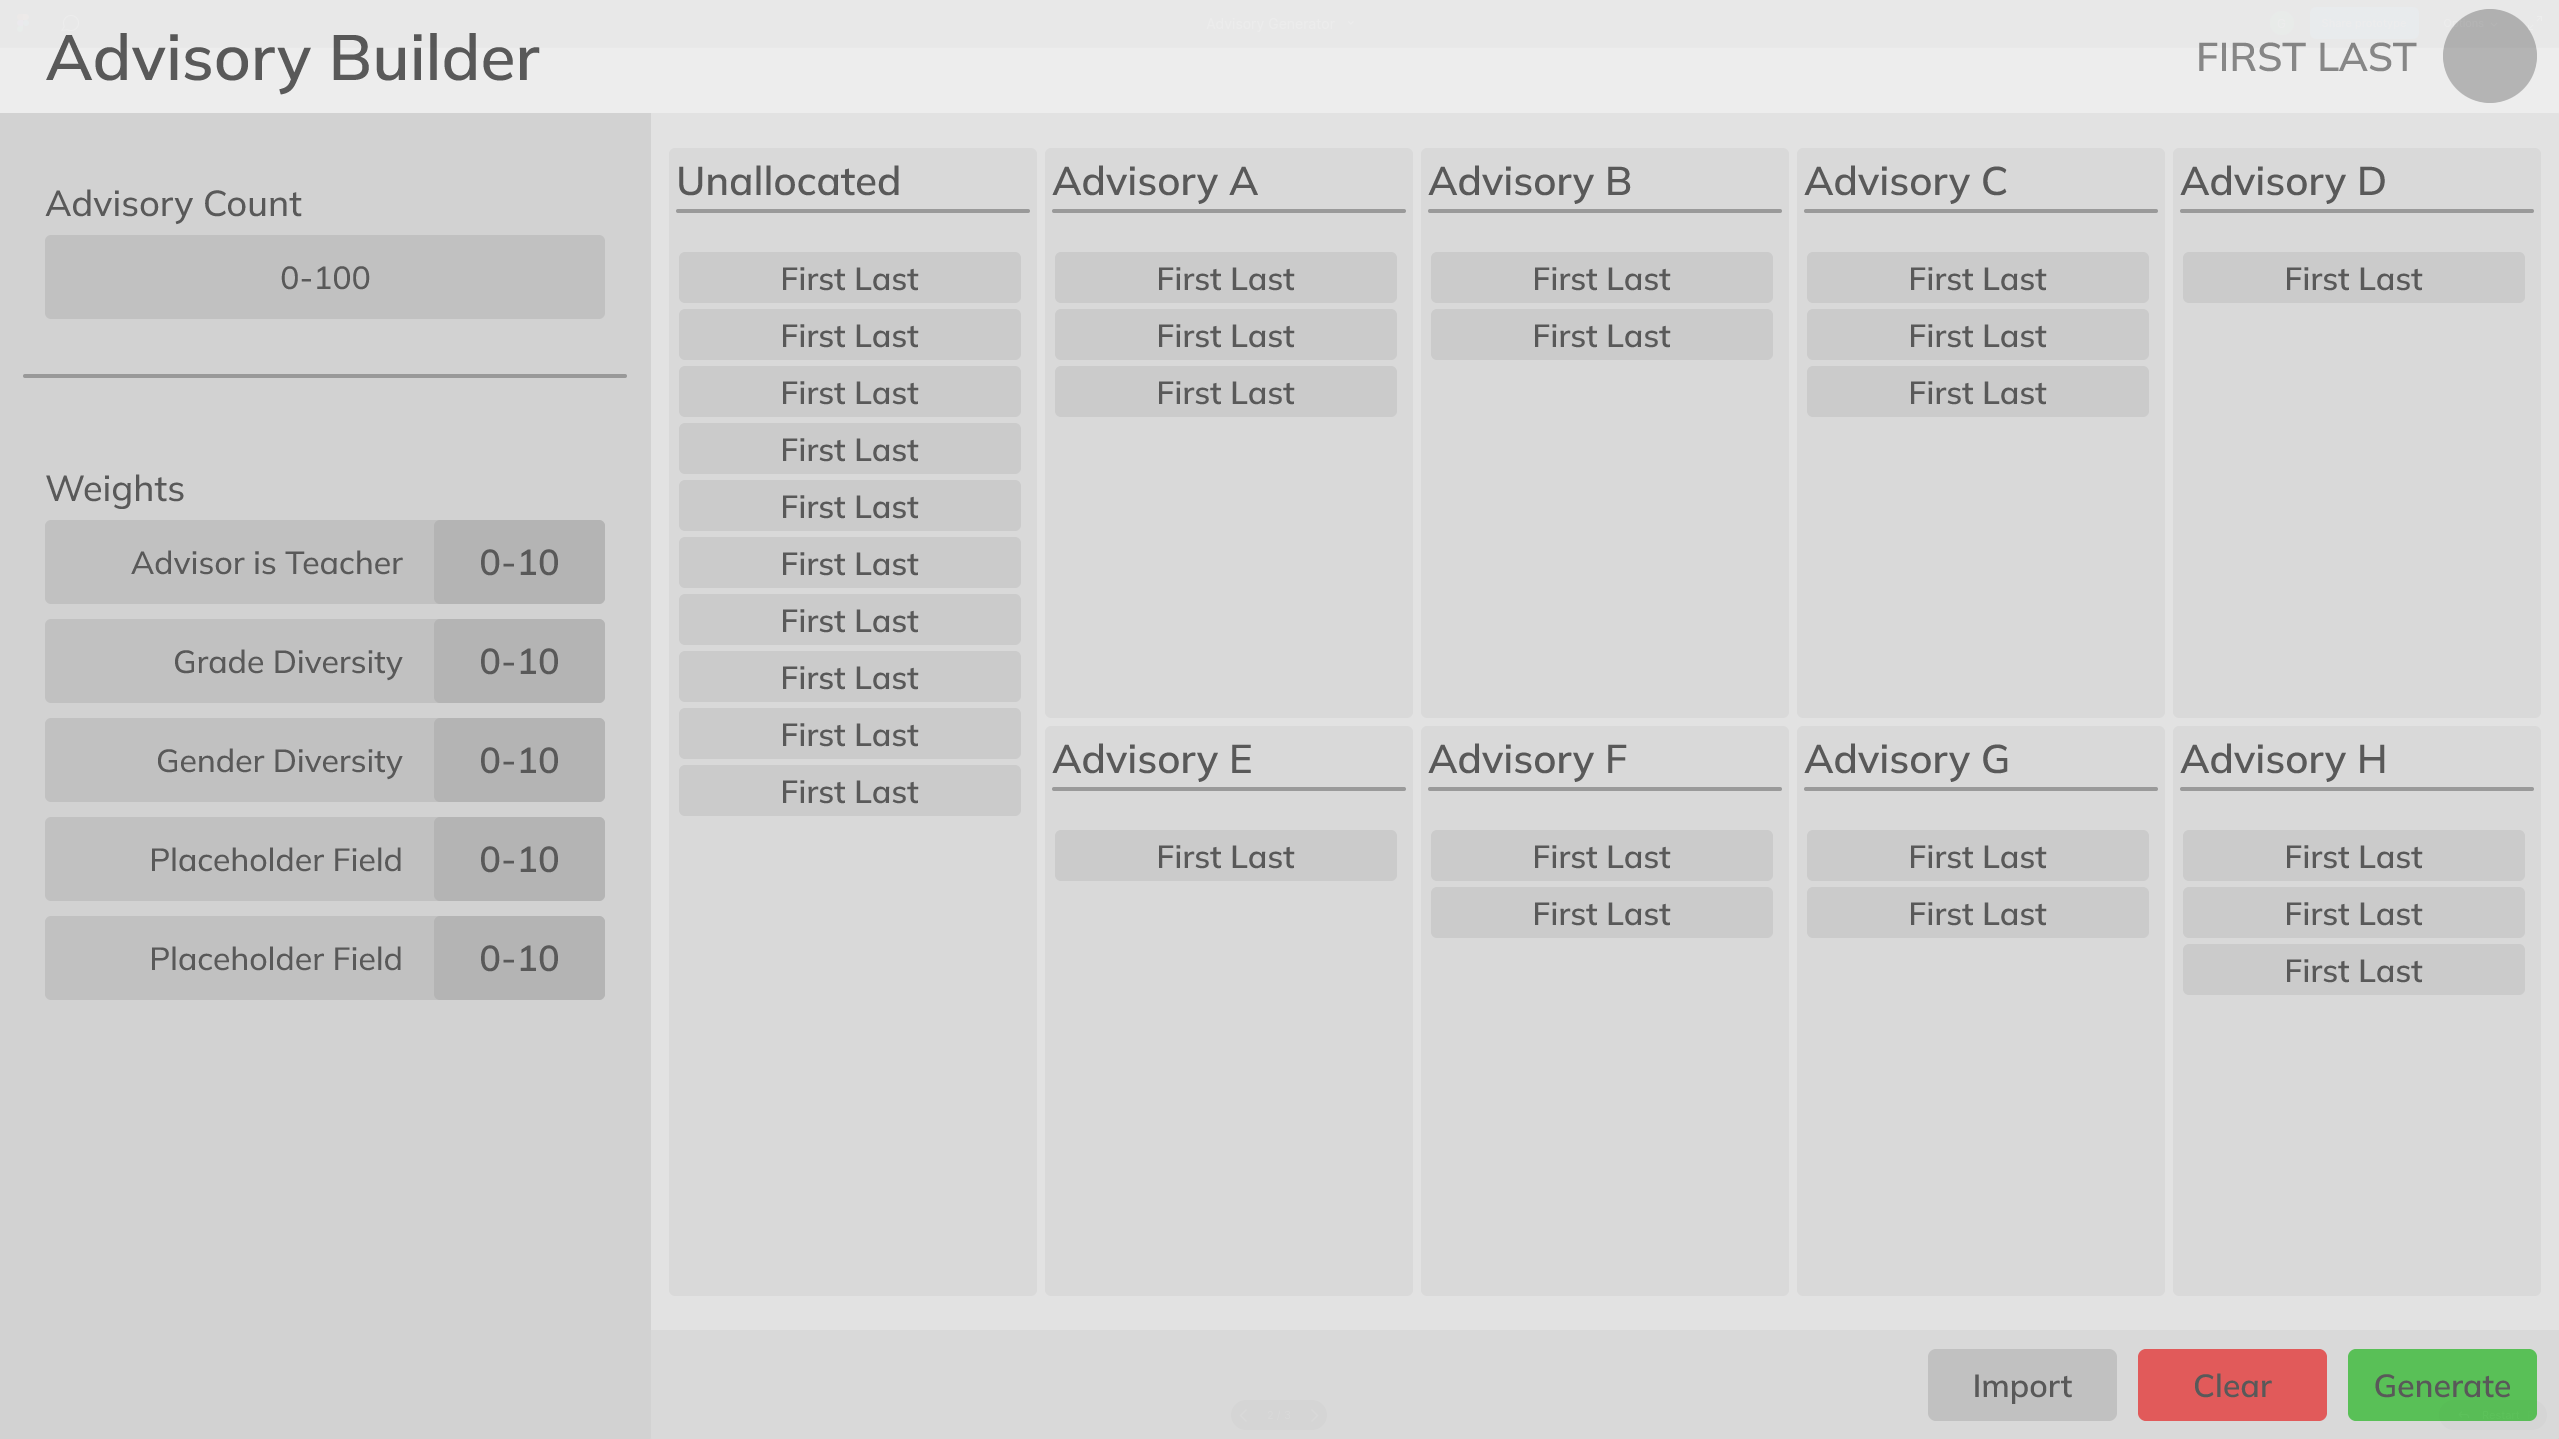
\includegraphics[width=\linewidth]{Dashboard-Mockup}
  \caption{Mockup of dashboard page showed to client}
  \label{design:dashboard}
\end{figure}
\begin{figure}
  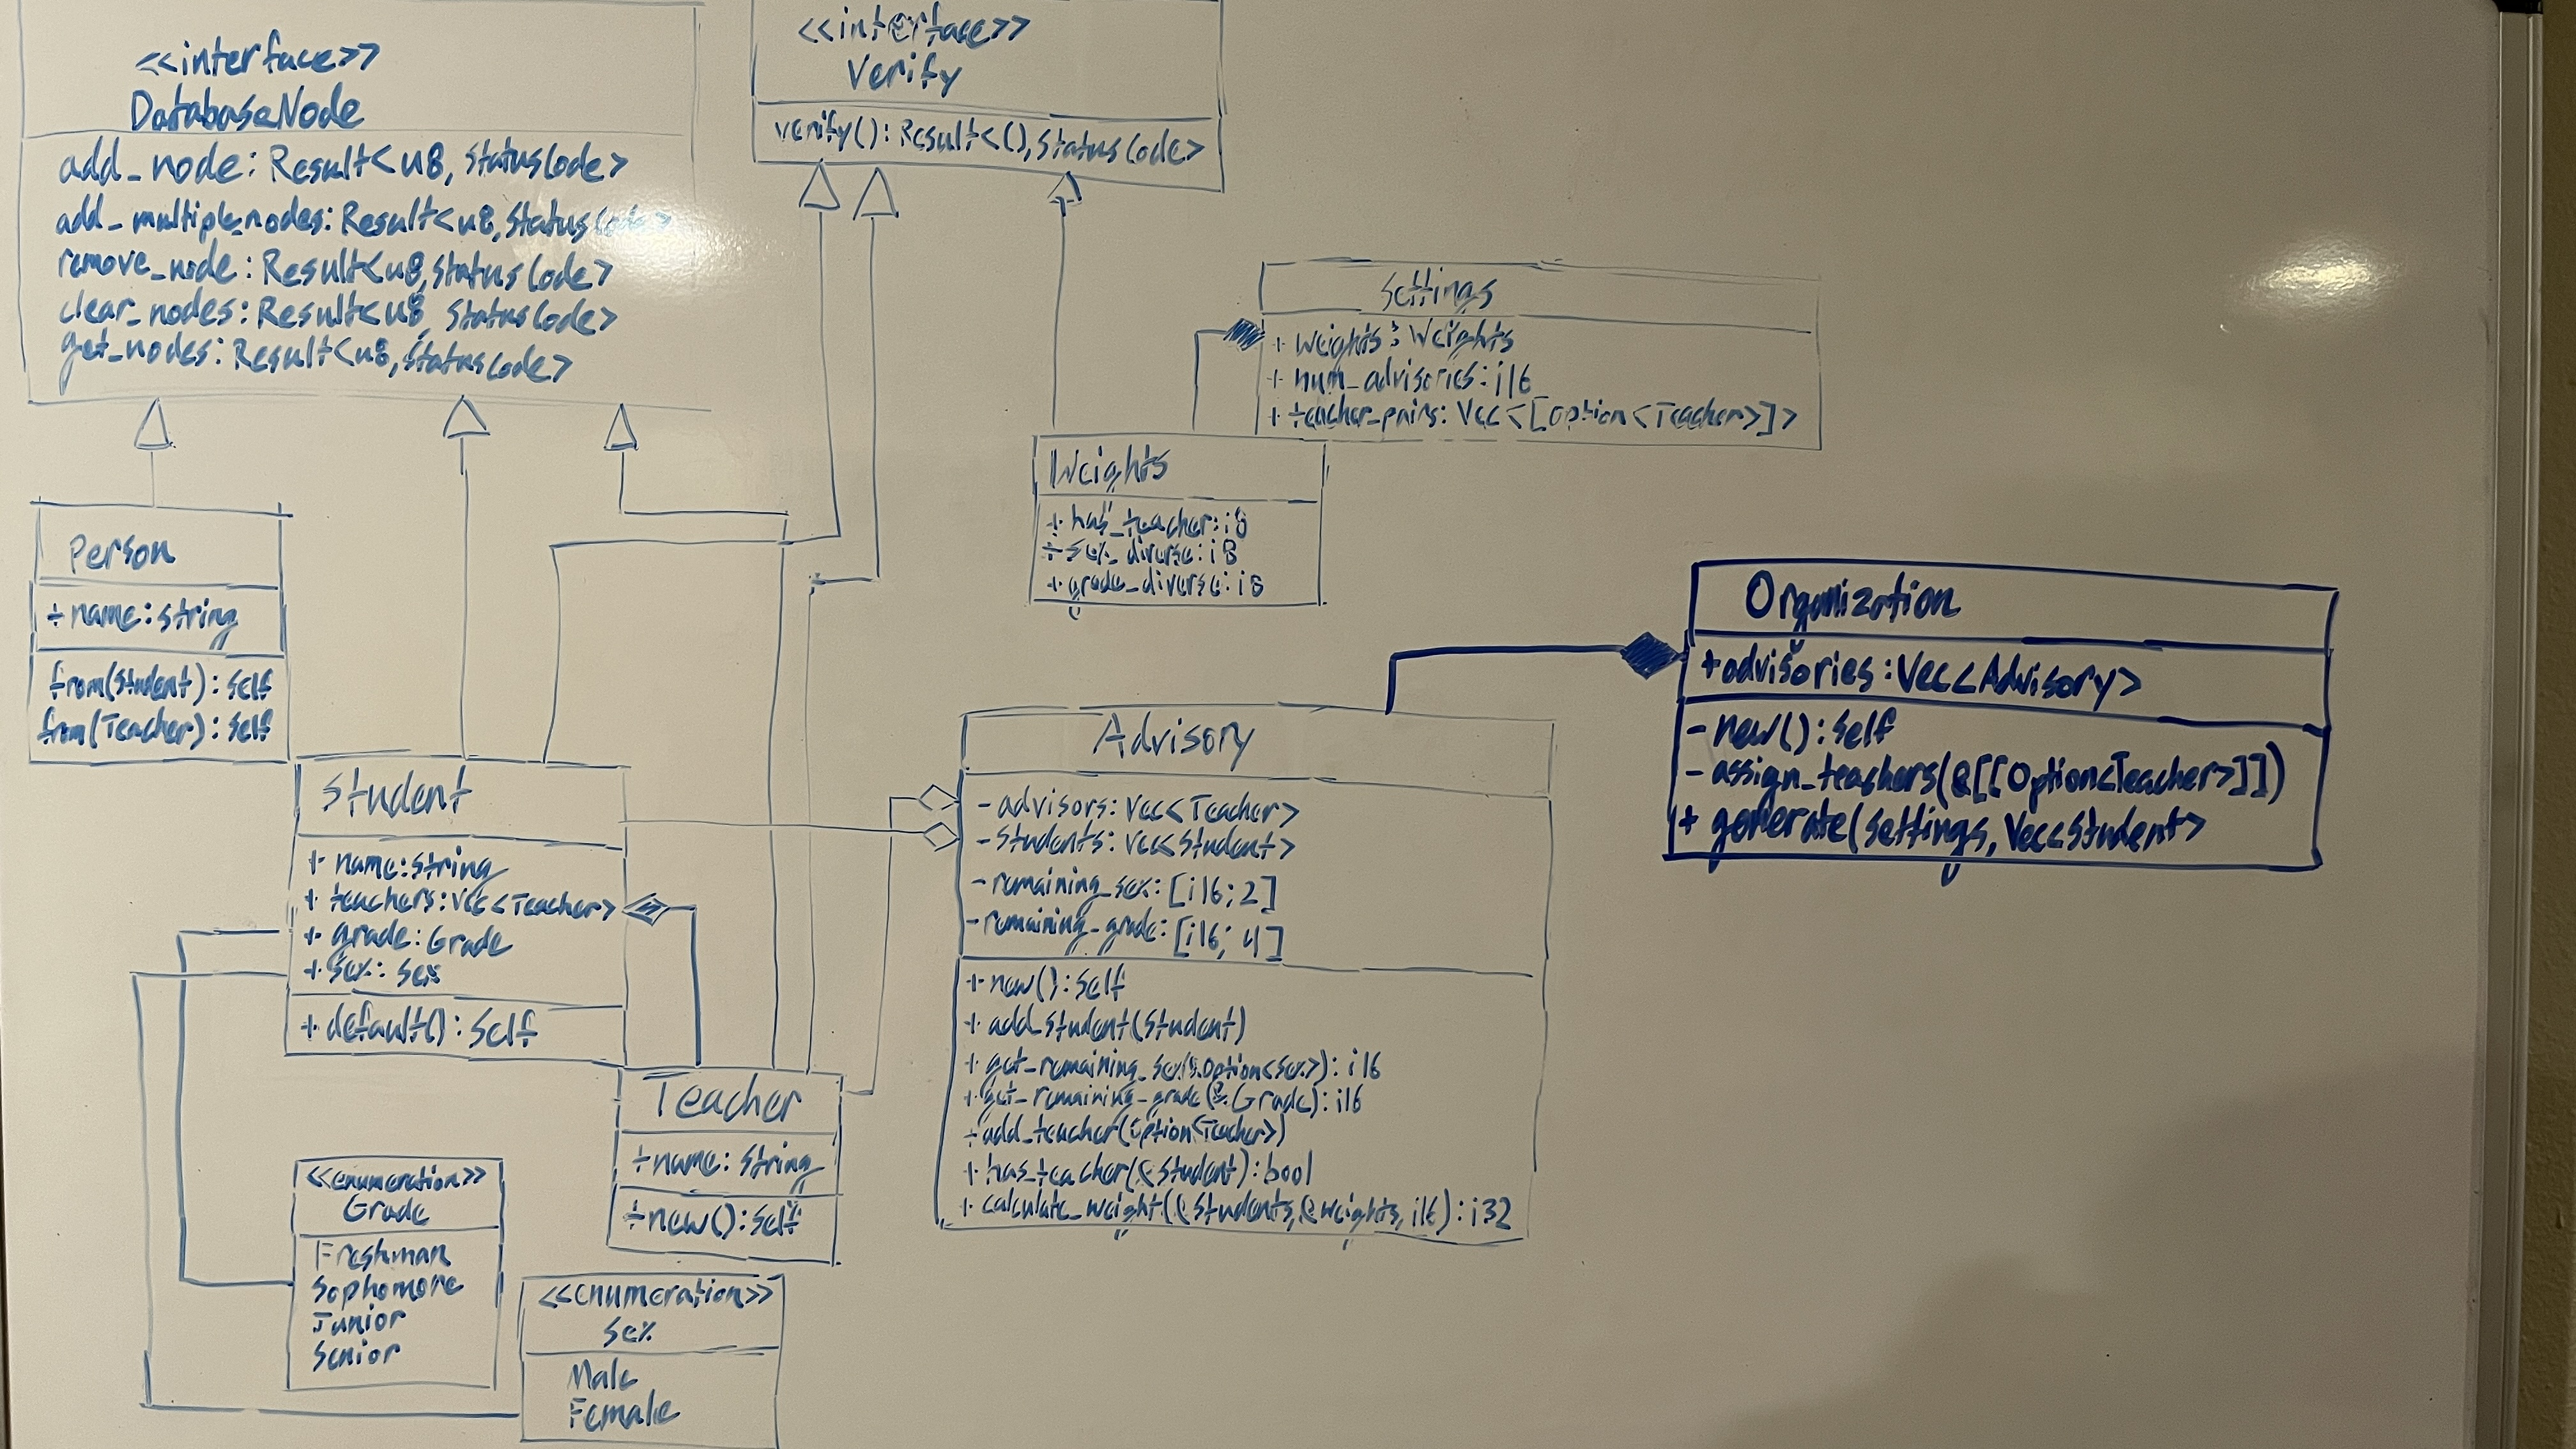
\includegraphics[width=\linewidth]{UML}
  \caption{UML diagram of backend structs, interfaces, and enums}
  \label{design:uml}
\end{figure}
\begin{figure}
  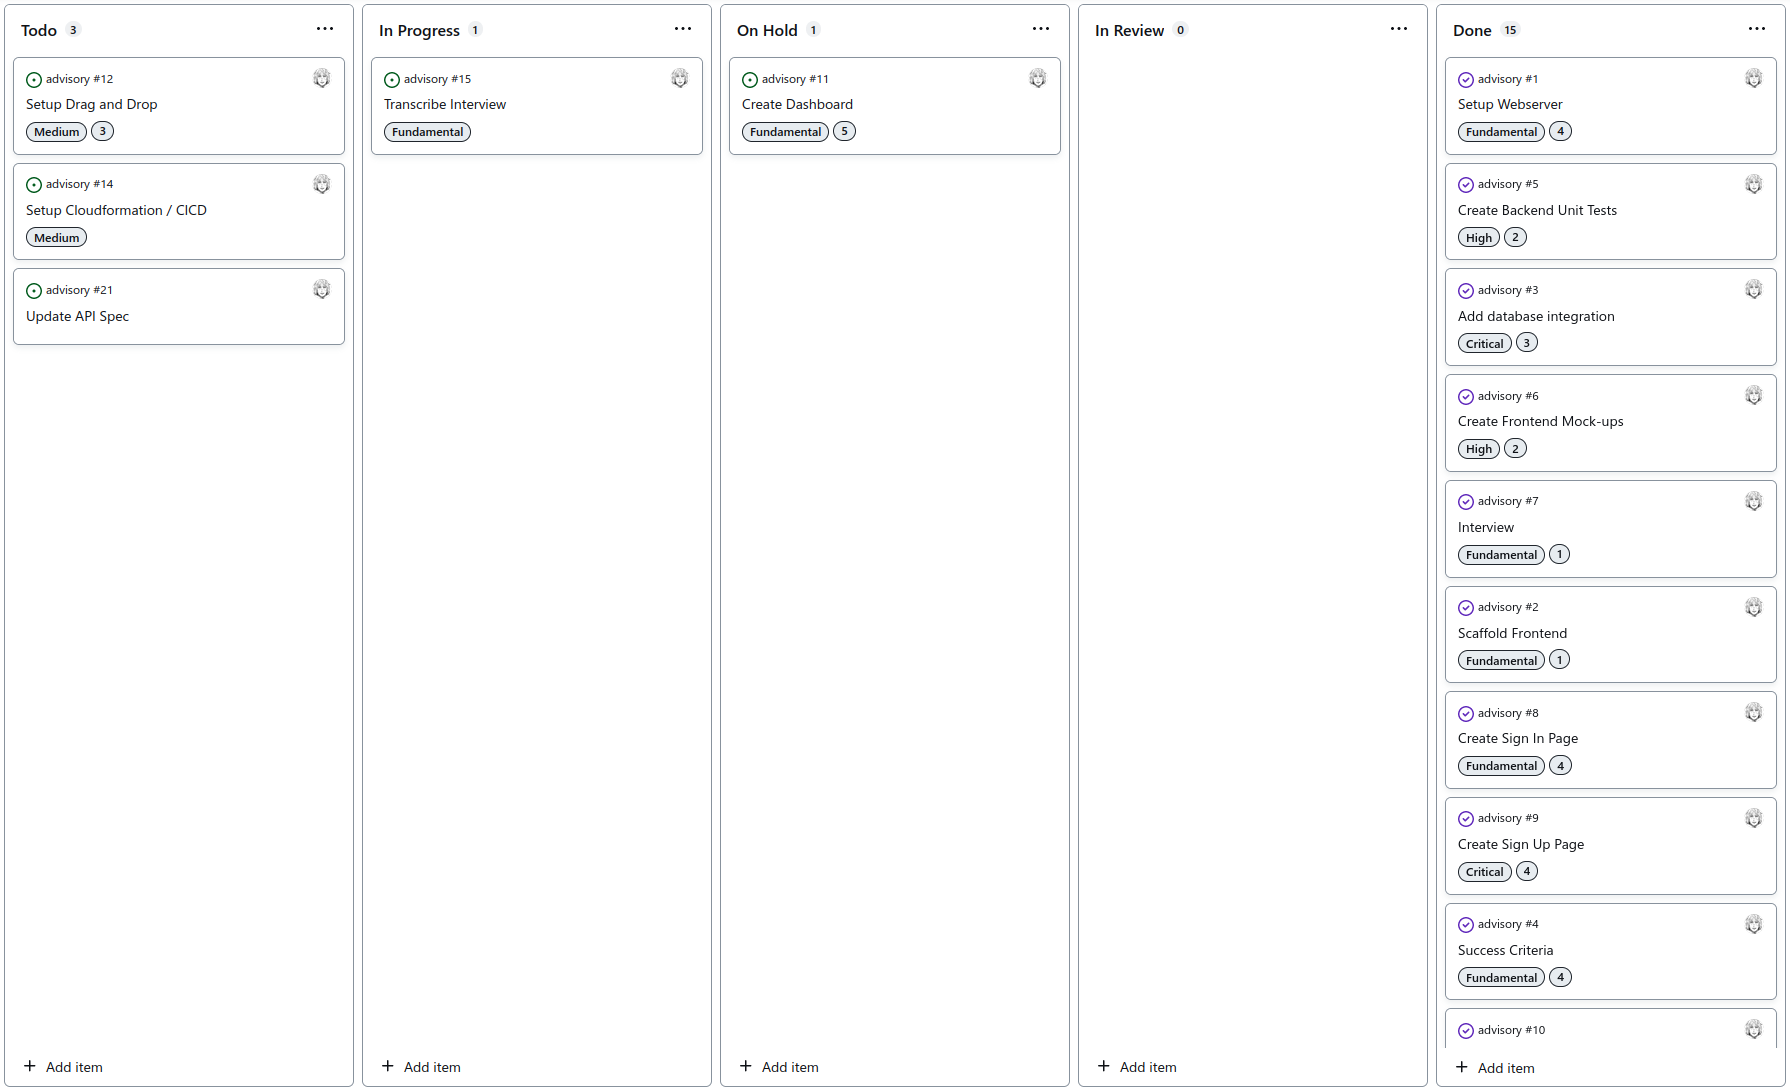
\includegraphics[width=\linewidth]{Github-Project-Board}
  \caption{Project board used for keeping track of tasks}
  \label{design:project_board}
\end{figure}

\section{Development}
\label{sec:develop}
After meeting with my client, I felt it most appropriate for the problem at hand---and in order to allow my client flexibility when using the tool---I decided to create a multi-layered application hosted on the cloud.
With my multi-layered architecture, the layers were established as the Frontend, Backend, and Database layers.
The Frontend is a static website with its assets hosted in an AWS S3 bucket.
The Backend is a webserver with a RESTful API implemented in Rust, containerized using Docker, and hosted on AWS Elastic Container Service deployed using AWS Fargate.
The Database is the Neo4j Graph Database, using an official docker image and similarly deployed to AWS ECS in order to communicate well with the Backend.
The development details for the Frontend and Backend are detailed in \cref{subsec:frontend,subsec:backend} respectively.

\subsection{Frontend}
\label{subsec:frontend}
Starting this project, the part I was most weary of was the Frontend.
I had created several Backends before, but had never ventured into CSS or Frontend frameworks.
At my summer internship, some of my fellow interns developed the frontend using React, which is considered the industry standard, but I wanted to try a developer-friendly framework I had heard about called Svelte.
My biggest challenges faced in this area were: working with CSS (especially making my website work on varying screen sizes) and the somewhat-limited Svelte ecosystem.
I wanted to use Google's Material UI (MUI) for on-screen assets such as buttons, text boxes, \&c, but found that the Svelte implementation of the standards, called SMUI, was poorly documented, rapidly evolving, and did not implement the MUI specifications completely.

As currently implemented, my Frontend is comprised of five pages, most of them for authentication purposes.
I implemented authentication and authorization using AWS Cognito User Pools.
A request is sent to AWS Cognito using a Javascript library, and the Frontend is returned a JSON web token that can be included in the Authentication header in future requests to the Backend.
As is, tokens are not stored in a cookie, though they persist between different pages of the site.
Using a cookie for the auth token is complicated because the token expires after a while, and the site would need to distinguish between a valid and expired token before refreshing.
This is an avenue for future improvement.

In order to allow my client to quickly add students and their relationships with their teachers, my product allows importing from a .xlsx spreadsheet.
This spreadsheet is created by school administration every year, and only needs the tweak of adding student sex in order to use.
The algorithm to extract data from the spreadsheet (once transformed to a 2d array) is shown in \cref{lst:import_students,lst:import_teachers}.
\cref{lst:import_students} (importing students) is significantly more complicated than \cref{lst:import_teachers} (importing teachers), as it needs to extract the student's teachers over multiple rows.
\cref{lst:import_students,lst:import_teachers} both use the Set datastructure in order to forbid duplicates.

\subfile{code/student_import}

\subfile{code/teacher_import}

The functional portion of the Frontend is a dashboard that allows for the user to tweak certain settings for the advisory generation program.
These settings are: number of generated advisories, and the relative weights of different factors in the generation process such as whether or not the advisory contains one of the student's teachers, grade diversity, and sex diversity.
These are sent to the Backend when the HTTP request to build the advisories is made.
These could be stored as a cookie or as a user-specific setting, but, similarly to the auth token, this is an avenue for future improvment to the product.

\subsection{Backend}
\label{subsec:backend}
The backend is significantly more complicated than the frontend, though it was easier for me to build.

The backend consists of an HTTP server that forwards requests to certain handlers based on path.
An example of a handler is \cref{lst:get_people_handler}.

\subfile{code/get_people_handler}

The handlers call methods of several different structs such as Student, Teacher, Person, Advisory, and Organization.
These methods handle the actual business logic of placing data from the frontend in the database, retrieving it, generating advisories, \&c.

\subsubsection{Core Logic}
The core logic for the product generates a group of advisories (refered to within the code as an \enquote{Organization}) using data from the.
The method relies on several other functions and methods in order to work, but the gist of its functionality is apparent in \cref{lst:generate}.
The method calculates a weighted value taking into account the relative weights set by the user on the Frontend between each Student and Advisory.
The algorithm then adds the student to the Advisory with the highest weighted value.
For the diversity weights (grade and sex,) each advisory has a quota for each possible sex \& grade.
The algorithm takes this into account and decreases or increases the weighted value in accordance with the remaining values for the quota.
Should the student be added to the some advisory, then the remaining quotas for their respective sex \& grade are decreased by one.

Pairs of students can be prevented from being placed in the same advisory through a specific path.
This creates a relationship in the graph database that is later stored in a vector on a per-student basis of all students that they should not be paired with.
When each student's weight for an advisory is being calculated, a method checks whether the advisory already contains one of the people that the student is banned from being placed with.
Should that be the case, the weighted value is reduced by 10,000, in order to effectively eliminate the chance of the student being placed in said advisory.

\subfile{code/generate}

\subsubsection{Refactor}
I built the backend twice, once just to get it working, then I refactored it to improve performance and readability.
In my refactor I made usage of more polymorphism through the use of \emph{traits}, a feature of Rust similar to interfaces in languages like Java.
Using this simplified my code and allowed for more structure.
\cref{lst:old_add_teacher} shows the pre-refactor code to add a teacher to the database.
Each struct that could be added to the database had an almost identical function, so I created a trait and simplified it to \cref{lst:new_add_teacher}.
\cref{lst:new_add_teacher} uses generics and is run as a method of Teacher using dot notation, versus in \cref{lst:old_add_teacher} where a Teacher object must be passed as a parameter.

\subfile{code/old_add_teacher}

\subfile{code/new_add_teacher}

Similar changes were made for many different functions, especially for those that interact with the database.

\section{Evaluation}
\label{sec:eval}


\label{mylastpage}
\newpage
\pagestyle{frontorback}
\pagenumbering{Roman}
\subfile{appendix}
\newpage
\listoffigures
\vspace{1cm}
\listofsnippets
\vspace{1cm}
\phantomsection
\addcontentsline{toc}{section}{References}
\printbibliography
\thispagestyle{frontorback}
\end{document}
